%automated figure captioning
\chapter{Background}

\section{Norway and SLEs in the Present Day}
 It would be reasonable to consider Norway's culture and socioeconomic position as dominated by its relationship with the sea. All of its major cities are located on the coast.  By January 2022, 31.6 percent of the Norway's coastal zone has been influenced by buildings, railways, roads and agriculture (\cite{engebakken_construction_2022}). This is notable as only 68.4 percent of the Norwegian coastline is currently deemed accessible due to its steep terrain (\cite{engebakken_construction_2022}). Norwegian weather is predicted to become more extreme (\cite{rod_integrated_2012}), in line with global trends, which project increasing coastal flooding due to extreme weather and sea-level rise (\cite{hoffken_effects_2020}). 
\paragraph{}

Due to settlement patterns in Norway and the changing climate, the threat of natural hazards related to the sea is increasing, which requires increased attention to be given to regional vulnerability and the resilience of places (\cite{opach_seeking_2020}; \cite{rod_three_2015}). Quantitative community resilience measurement approaches have been tried, but there are several limiting factors including that they rarely offer policy makers the strategies required for building resilience (\cite{opach_seeking_2020}; \cite{gerkensmeier_governing_2018}). Important information can be gained from vulnerability indices, including better understanding of social vulnerability, but questions remain about how social vulnerability can be decrease to build resilience. 


\section{Introduction to Research Area}

Trondheim is situated deep within Trondheimsfjord, which protects it from the North Sea (figure \ref{fig:research_area}). The maximum observed sea level extreme in Trondheim is 2.06m (referring to elevation reference model NN2000), recorded in 1971 (\cite{kartverket_high_2022}). Trondheim municipality plans indicate that the city should be prepared for SLEs of 4.87m by 2100. 
\paragraph{}
Trondheim can be considered one of the most resilient places in Norway due to its protected location, geological setting, infrastructure and socioeconomic status (\cite{opach_seeking_2020}). Thus, it would be reasonable to assume that unlike other places in Norway the infrastructure in Trondheim is not at risk from SLEs (\cite{baisotti_farevarsel_2020}). Such an assumption can be backed up by the knowledge of the fact that the Earth's crust below Norway is still rebounding due to deglaciation following the last ice age; a process known as glacioisostatic adjustment (\cite{breili_high-accuracy_2020}). What is perhaps less widely understood, is that glacioisostatic adjustment is an incredibly varied process across the country and the basic model that the majority of the population has about sea level-rise and land uplift, may be creating a false confidence, especially as weather events due to their uncertainty are often excluded from sea level rise projections  (\cite{breili_high-accuracy_2020}, \cite{hanssen-bauer_climate_2017}).  Furthermore the tidal patterns in Trondheimsfjord (\ref{fig:research_area}) are complex, as is often the case in deep fjords, adding another layer of uncertainty to the projections of changing sea levels (\cite{hanssen-bauer_climate_2017}).

\begin{figure}[H]
    \centering
    \includegraphics[width=1.0\textwidth]{fig/Trondheimsfjord.png}
    \caption[Research area - Trondheimsfjord]
    {The city of Trondheim is situated in Trondheimsfjord, which provides protection from the North Sea. The red line represents Norway's major road network. The E6, perhaps the most critical road infrastructure for Trondheim is shown as close to the coast. Figure created using ArcGIS Pro. }
    \label{fig:research_area}
    
\end{figure}



\section{Study Sites} \label{study-sites-background}
Four study sites situated on Trondheim's coast were chosen for their high daily population throughput, large amounts of infrastructure, and coastal characteristics. These are Brattøra, Grillstad, Skansen and Nidelva. Physical vulnerability to SLEs is diverse for these sites, as can be seen in figure ~\ref{fig:research_site} below and is further outlined in table ~\ref{table:research_site}. 
\paragraph{}

\begin{figure} [H]
    \centering
    \includegraphics[width=1.0\textwidth]{fig/trondheim_research_sites_grey_circles.png}
    \caption[Research sites - Trondheim]{The sites chosen to investigate Trondheim are Brattøra, Grillstad, Skansen and Nidelva. These sites are highlighted with a purple circle. As shown here Brattøra has both the sea, canal and a section of artificially straightened tidal river within its site. Grillstad includes reclaimed land and an artificial island connected via a bridge. Nidelva takes its name from the river running through it. It is further from the open fjord , but includes marinas. Skansen has the sea and canal within its site, while its river is not straightened it is prevented from shifting. Figure was created using ArcGIS Pro.}
    \label{fig:research_site}
\end{figure}

\paragraph{}


Factors considered in defining physical vulnerability to sea-level rise (including SLEs) are: natural resistance to erosion, engineered resistance to erosion, engineered protection to SLEs, infrastructure built directly upon coastline, settlement patterns, usage patterns and projected changes in SLEs. The physical vulnerability was determined from direct observation,  models from \cite{kartverket_se_2021} and consulting planning documents for each site (\cite{miljoenheten_og_byplankontoret_trondheim_kommune_9-notat-om-havnivastigning-og-stormflo---hensyn-i-arealplanlegging-nyhavnapdf_2020}). 


\paragraph{}
\begin{table}[!ht]
    \centering
    \begin{tabular}{|l|l|l|l|l|}
    \hline
        \textbf{location} & \textbf{Brattøra} & \textbf{Grillstad} & \textbf{Skansen}  & \textbf{Nidelva} \\ \hline
        PV 70 years ago & high & high & medium & Low \\ \hline
        PV now &  medium &  medium &  low &  low \\ \hline
        PV in 70 years &  high &  high &  medium &  medium \\ \hline
        Dominant & Office space  & Residential & Recreational  & Residential and \\ \newline
        use & and harbour &  only   &  and industry & and commercial  \\ \hline
        Land type & Reclaimed land & Reclaimed land & Managed coastline  & Altered tidal river \\ \hline
        protection & Harbour wall & Harbour wall & Harbour wall, placed rocks & inland \\ \hline
    \end{tabular}
    \caption{ Research Sites Changing Physical Vulnerability to SLEs}{Created from observation of the sites conducted in 2021 and \cite{kartverket_se_2021}}
    \label{table:research_site}
\end{table}

Brattøra is the research site with the least amount of residential population. Most buildings are occupied by offices and are protected by a harbour wall and a small harbour behind that (figure \ref{fig:research_site}). Brattøra is located on reclaimed land and for this reason it had a very high physical vulnerability to sea-level rise and SLEs 70 years ago. The modern harbour and area's design have lowered the physical vulnerability to medium now, but it is projected to have several areas that are flooded regularly by the 2090s (\cite{kartverket_se_2021}). Currently, the vulnerable areas in Brattøra are predominantly sustainable urban development schemes with footpaths and car parks located where the majority of current potential flooding would occur. However, there is still risk of more significant impacts from SLEs beyond nuisance flooding, such as erosion, disconnecting important transport routes (figure \ref{fig:research_site}) and preventing access to offices.
\paragraph{}
Grillstad is also located on reclaimed land, and like Brattøra, had a very high physical vulnerability 70 years ago. It is also located behind a harbour, including a harbour wall now, but in contrast to  Brattøra, the dominant land use is residential (Table \ref{table:research_site}). There are several small commercial ventures, but the vast majority serve the needs only of local residents. There are no major transport connections or industry at this site. 
\paragraph{}
Nidelva is a less obvious choice for research into SLEs as it is situated further from the coastline. The land type here is altered tidal river and its physical vulnerability 70 years ago was low. The dominant uses are residential and commercial and it has lower physical vulnerability predicted in 70 years than Brattøra and Grillstad (Table \ref{table:research_site}). The Nidelva study area has the added complication of the river level potentially impacting the height of the water at certain times. The river here is controlled by the dam in Leirfoss, which is part of the hydroelectric power scheme which provides energy to the area.
\paragraph{}
Skansen has two dominant uses of recreation and industry, however, there is also significant residency in the area, the majority being high-rise apartment buildings at least 10m from the coastline. While several aspects of this coastline may appear more natural, it is a managed coastline which is protected by placed rocks, a harbour wall and small bays. Unlike the other sites, there have been attempts to utilise natural techniques to prevent flooding in this area. This includes the restoration of Illabekken river and banks and the use of so-called living shorelines, in this case non-concreted areas which are covered in plants to improve infiltration (\cite{selliseth_ilabekken_2021}.
\paragraph{}

\paragraph{}
Brattøra, Skansen and Nidelva have previously been highlighted during case presentations by the municipality as areas that currently have a risk of temporary flooding (\cite{hanssen_saksframlegg_2013}). This risk level is projected to change over the next 100 years (\cite{hanssen-bauer_climate_2017}). This is why these areas have special building requirements such as water-tight basements and keeping electrical installations above the area of potential flooding (\cite{hanssen_saksframlegg_2013}). Grillstad was not specified in the report as it was built after publication, but it is located in the area requiring special building requirements so it can also be considered a vulnerable area. 







\section{ Natural System Resilience}

The datasets  \cite{geonorge_stormflo_2021} , \cite{kartverket_se_2021}, \cite{stormflo_database_stormflo_2021} and \cite{ipcc_sea_2021} were used to create visual simulations and maps of SLEs, which supported the research of the determination of Trondheim's resilience. 

\section{Visual Simulation of SLEs} \label{visual-simulations}
 Figures ~\ref{fig:SLE-nidelva} to ~\ref{fig:sle-skansen} display the simulated SLEs created for this project. 

\begin{figure}[H]
    \centering
    \includegraphics[width=16cm]{fig_sle/nidelva 2090 q.png}
    \caption{Simulated SLEs for Nidelva}
    {These were created using Inkscape and GIMP.}
    \label{fig:SLE-nidelva}
\end{figure}

\begin{figure}[H]
    \centering
    \includegraphics[width=16cm]{fig_sle/boxes top left - brattora sle.png}
    \caption{Simulated SLEs for Brattøra}
    {These were created using Inkscape and GIMP. }
    \label{fig:SLE-brattora}
\end{figure}

\begin{figure}[H]
    \centering
    \includegraphics[width=16cm]{fig_sle/grillstad 2090 q.png}
    \caption{Simulated SLEs for Grillstad}{These were created using Inkscape and GIMP. }
    \label{fig:SLE-grillstad}
\end{figure}

\begin{figure}[H]
    \centering
    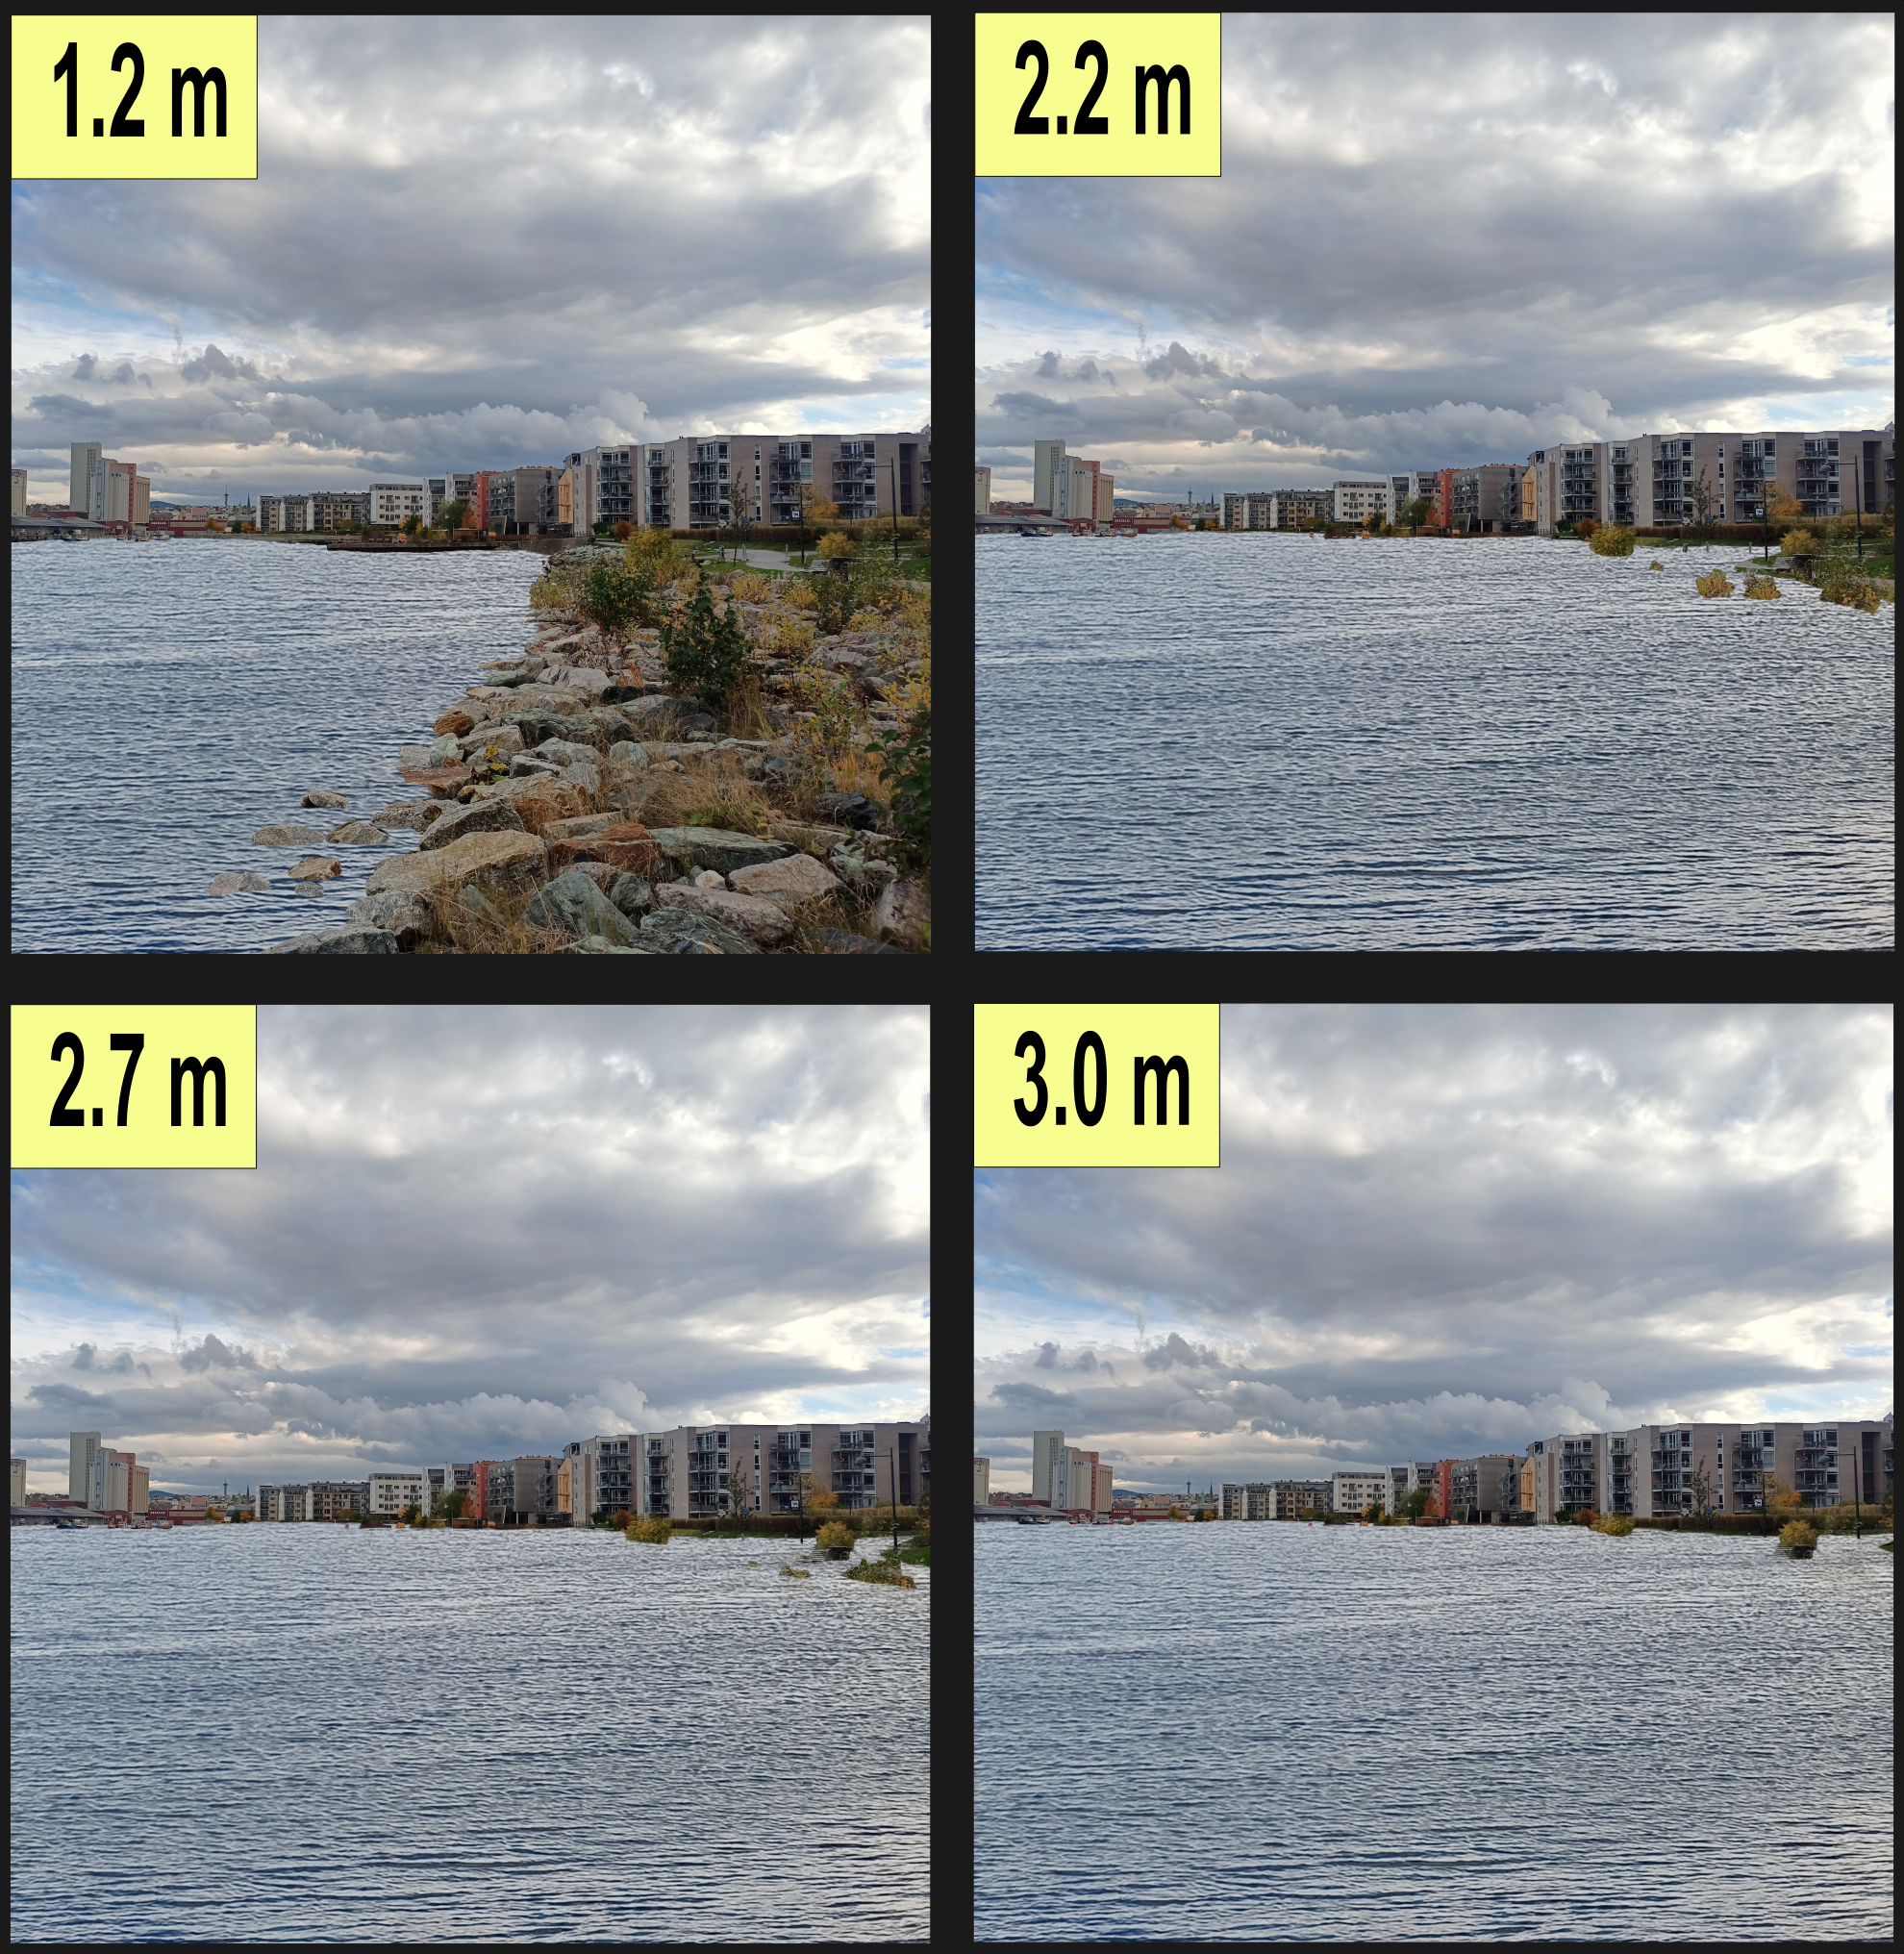
\includegraphics[width=16cm]{fig_sle/illsvika 2090 q.png}
    \caption{Simulated SLEs for Skansen}{These were created using Inkscape and GIMP. }
    \label{fig:sle-skansen}
\end{figure}


The differing heights represent different potential events. The top left square, 1.2m is a very likely event as this is the height associated with the spring high tide for each of the research sites. The top right square, 2.2m is a significantly less likely as it represents the water level height associated with the current 20 year storm surge, while a water level of 2.7m is projected for the 20 year storm surge in 2090. Finally, the 1000 year storm surge in 2090 is represented by 3.0m as seen in the bottom right square of each of the figures. The figures also display how natural systems interplay with technological systems.

\section{Maps of SLEs}
Figures ~\ref{fig:sle_skansen_num} to ~\ref{fig:sle_nidelva_num}  display the mapped SLEs created for this thesis based off \cite{kartverket_se_2021} and \cite{stormflo_database_stormflo_2021}, across the same four research sites.

\begin{figure}[H]
    \centering
    \includegraphics[width=16cm]{fig_sle/skansen-sle-num.png}
    \caption{Projected SLEs for Skansen}{These were created using \cite{kartverket_se_2021} and \cite{stormflo_database_stormflo_2021}. }
    \label{fig:sle_skansen_num}
\end{figure}

\begin{figure}[H]
    \centering
    \includegraphics[width=16cm]{fig_sle/brattora-sle-num-bigger-boxes.png}
    \caption{Projected SLEs for Brattøra}{ These were created using \cite{kartverket_se_2021} and \cite{stormflo_database_stormflo_2021}. }
    \label{fig:sle_brattora_num}
\end{figure}

\begin{figure}[H]
    \centering
    \includegraphics[width=16cm]{fig_sle/grillstad-sle-num.png}
    \caption{Projected SLEs for Skansen}{ These were created using \cite{kartverket_se_2021} and \cite{stormflo_database_stormflo_2021}. }
    \label{fig:sle_grillstad_num}
\end{figure}

\begin{figure}[H]
    \centering
    \includegraphics[width=16cm]{fig_sle/nidelva-sle-num.png}
    \caption{Projected SLEs for Skansen}{These were created using \cite{kartverket_se_2021} and \cite{stormflo_database_stormflo_2021}. }
    \label{fig:sle_nidelva_num}
\end{figure}

 Bridges were not well included in the original models; as all bridges were marked as being flooded at every sea level extreme, which was not in line with the numerical values. The bridges in these maps have been adjusted to more accurately match the sea level extreme represented. The differing heights represent different potential events,  as described with the edited photographs shown in the section above. 

\section{Technological Systems Resilience}
Distinguishing technological and natural systems can be difficult in a landscape which has been actively shaped by its population for as long as Trondheim. Trondheim has been populated since the stone age and a major population site for over 1000 years (\cite{sjavik_z_2010}). For this thesis the understanding of technological system resilience focuses upon infrastructure in the four study areas, especially the location buildings and roads. How this infrastructure is built is of course of great importance to whether a speedy return to normality is possible after a sea level extreme event. Norway has strict building regulations, with additional rules about infrastructure in vulnerable locations (\cite{direktoratet_for_byggkvalitet_direktoratet_2016}). Yet, even very well-designed infrastructure will still be impacted if flooded. Impacts range from the obvious prevention of use during flooding, to post-event clean up and the wear and damage which can occur due to  erosion around building foundations, wave abrasion and salt-water damage.
\paragraph{}
Table ~\ref{table:building-impact-sle} displays the number of buildings which are likely to be impacted during different SLEs in Trondheim. This was modelled by \cite{kartverket_se_2021} and was the base of later water level simulations as used in this project. Importantly, the models from \cite{kartverket_se_2021} are more localised than previous models of SLEs in Norway.

\begin{table}[H]
    \centering
    \begin{tabular}{|l|l|l|l|l|}
    \hline
        \textbf{projected SLEs }& \textbf{No. Buildings}  & ~ & ~ & ~ \\ \hline
        ~ & Private & Private & Public  & Critical  \\ \newline
        ~ & Buildings & Businesses & Buildings & Buildings \\ \hline        
        20 years return height 2022 & 160 & 77 & 10 & 0 \\ \hline
        200 years return height 2022 & 214 & 87 & 10 & 0 \\ \hline
        1000 years return height 2022 & 242 & 104 & 14 & 0 \\ \hline
        Flooded 2090 & 66 & 51 & 8 & 0 \\ \hline
        20-years return height 2090 & 264 & 119 & 17 & 1 \\ \hline
        200-years return height  2090 & 308 & 136 & 24 & 1 \\ \hline
        1000-years return height  2090 & 332 & 148 & 26 & 1 \\ \hline
        1m sea level rise & 127 & 64 & 9 & 0 \\ \hline
        2m sea level rise & 343 & 155 & 29 & 1 \\ \hline
        3m sea level rise & 584 & 285 & 55 & 3 \\ \hline
        4m sea level rise & 752 & 335 & 70 & 5 \\ \hline
        5m sea level rise & 1023 & 402 & 77 & 8 \\ \hline
    \end{tabular}
    \caption{Impact of SLEs to Buildings in Trondheim }{translated from \cite{kartverket_se_2021}. Critical building are those which are critical to the function of the community such as hospitals. Explanation of "years return height" is available in section \ref{theory-nature-tech-resilience} }
    \label{table:building-impact-sle}
\end{table}


Table ~\ref{table:building-impact-sle} shows that there is currently some risk from SLEs to buildings in Trondheim, now and in the future. For example, the projected 20 year return height - 2022 is expected to cause the flooding of 247 buildings in total. Additionally, the table shows the number of buildings projected to flood at different projected SLEs. The major contrast between the 20 year return height - 2022 and the 20 year return height - 2090 is that the water level is high enough to flood a critical building, such as hospitals . Flooding of a critical building would also occur at 2m sea level rise. It is projected by 2090 that 115 building will be continuously flooded.
